%%%%%%%%%%%%%%%%%%%%%%%%%%%%%%%%%%%%%%%%%%%%%%%%%%%%%%
\chapter{Integrated experimental strategy}
\label{experimental_design}
\graphicspath{{chapter_03/figures}{chapter_03/tables}}
%%%%%%%%%%%%%%%%%%%%%%%%%%%%%%%%%%%%%%%%%%%%%%%%%%%%%%


This chapter outlines the integrated experimental strategy designed to address the research questions presented in Chapter \ref{general_introduction}, thereby providing a proof of concept for medium-range predictions of areas at risk of flash floods across a continuous global domain. The strategy follows a \textit{three-research-component approach}, where each component builds upon the findings of the previous ones (Figure \ref{fig:integrated_experimental_strategy}, rows related to \textit{research questions} and \textit{research components}). 

The \marginpara{First research component (addressing RQ1): development of a flash-flood-focused verification framework to assess predictions of areas at risk of flash flood} first research component addresses the development of a flash-flood-focused verification framework for rainfall forecasts, designed to benchmark the capability of medium-range global NWP rainfall forecasts to identify areas at risk of flash floods. This verification framework serves two critical purposes: it first establishes a baseline of how effectively state-of-the-art global NWP models predict rainfall patterns associated with flash flood risk up to medium-range lead times. Second, it provides a benchmark against which more sophisticated predictive systems can be evaluated.

\begin{figure}[htbp]
\centering
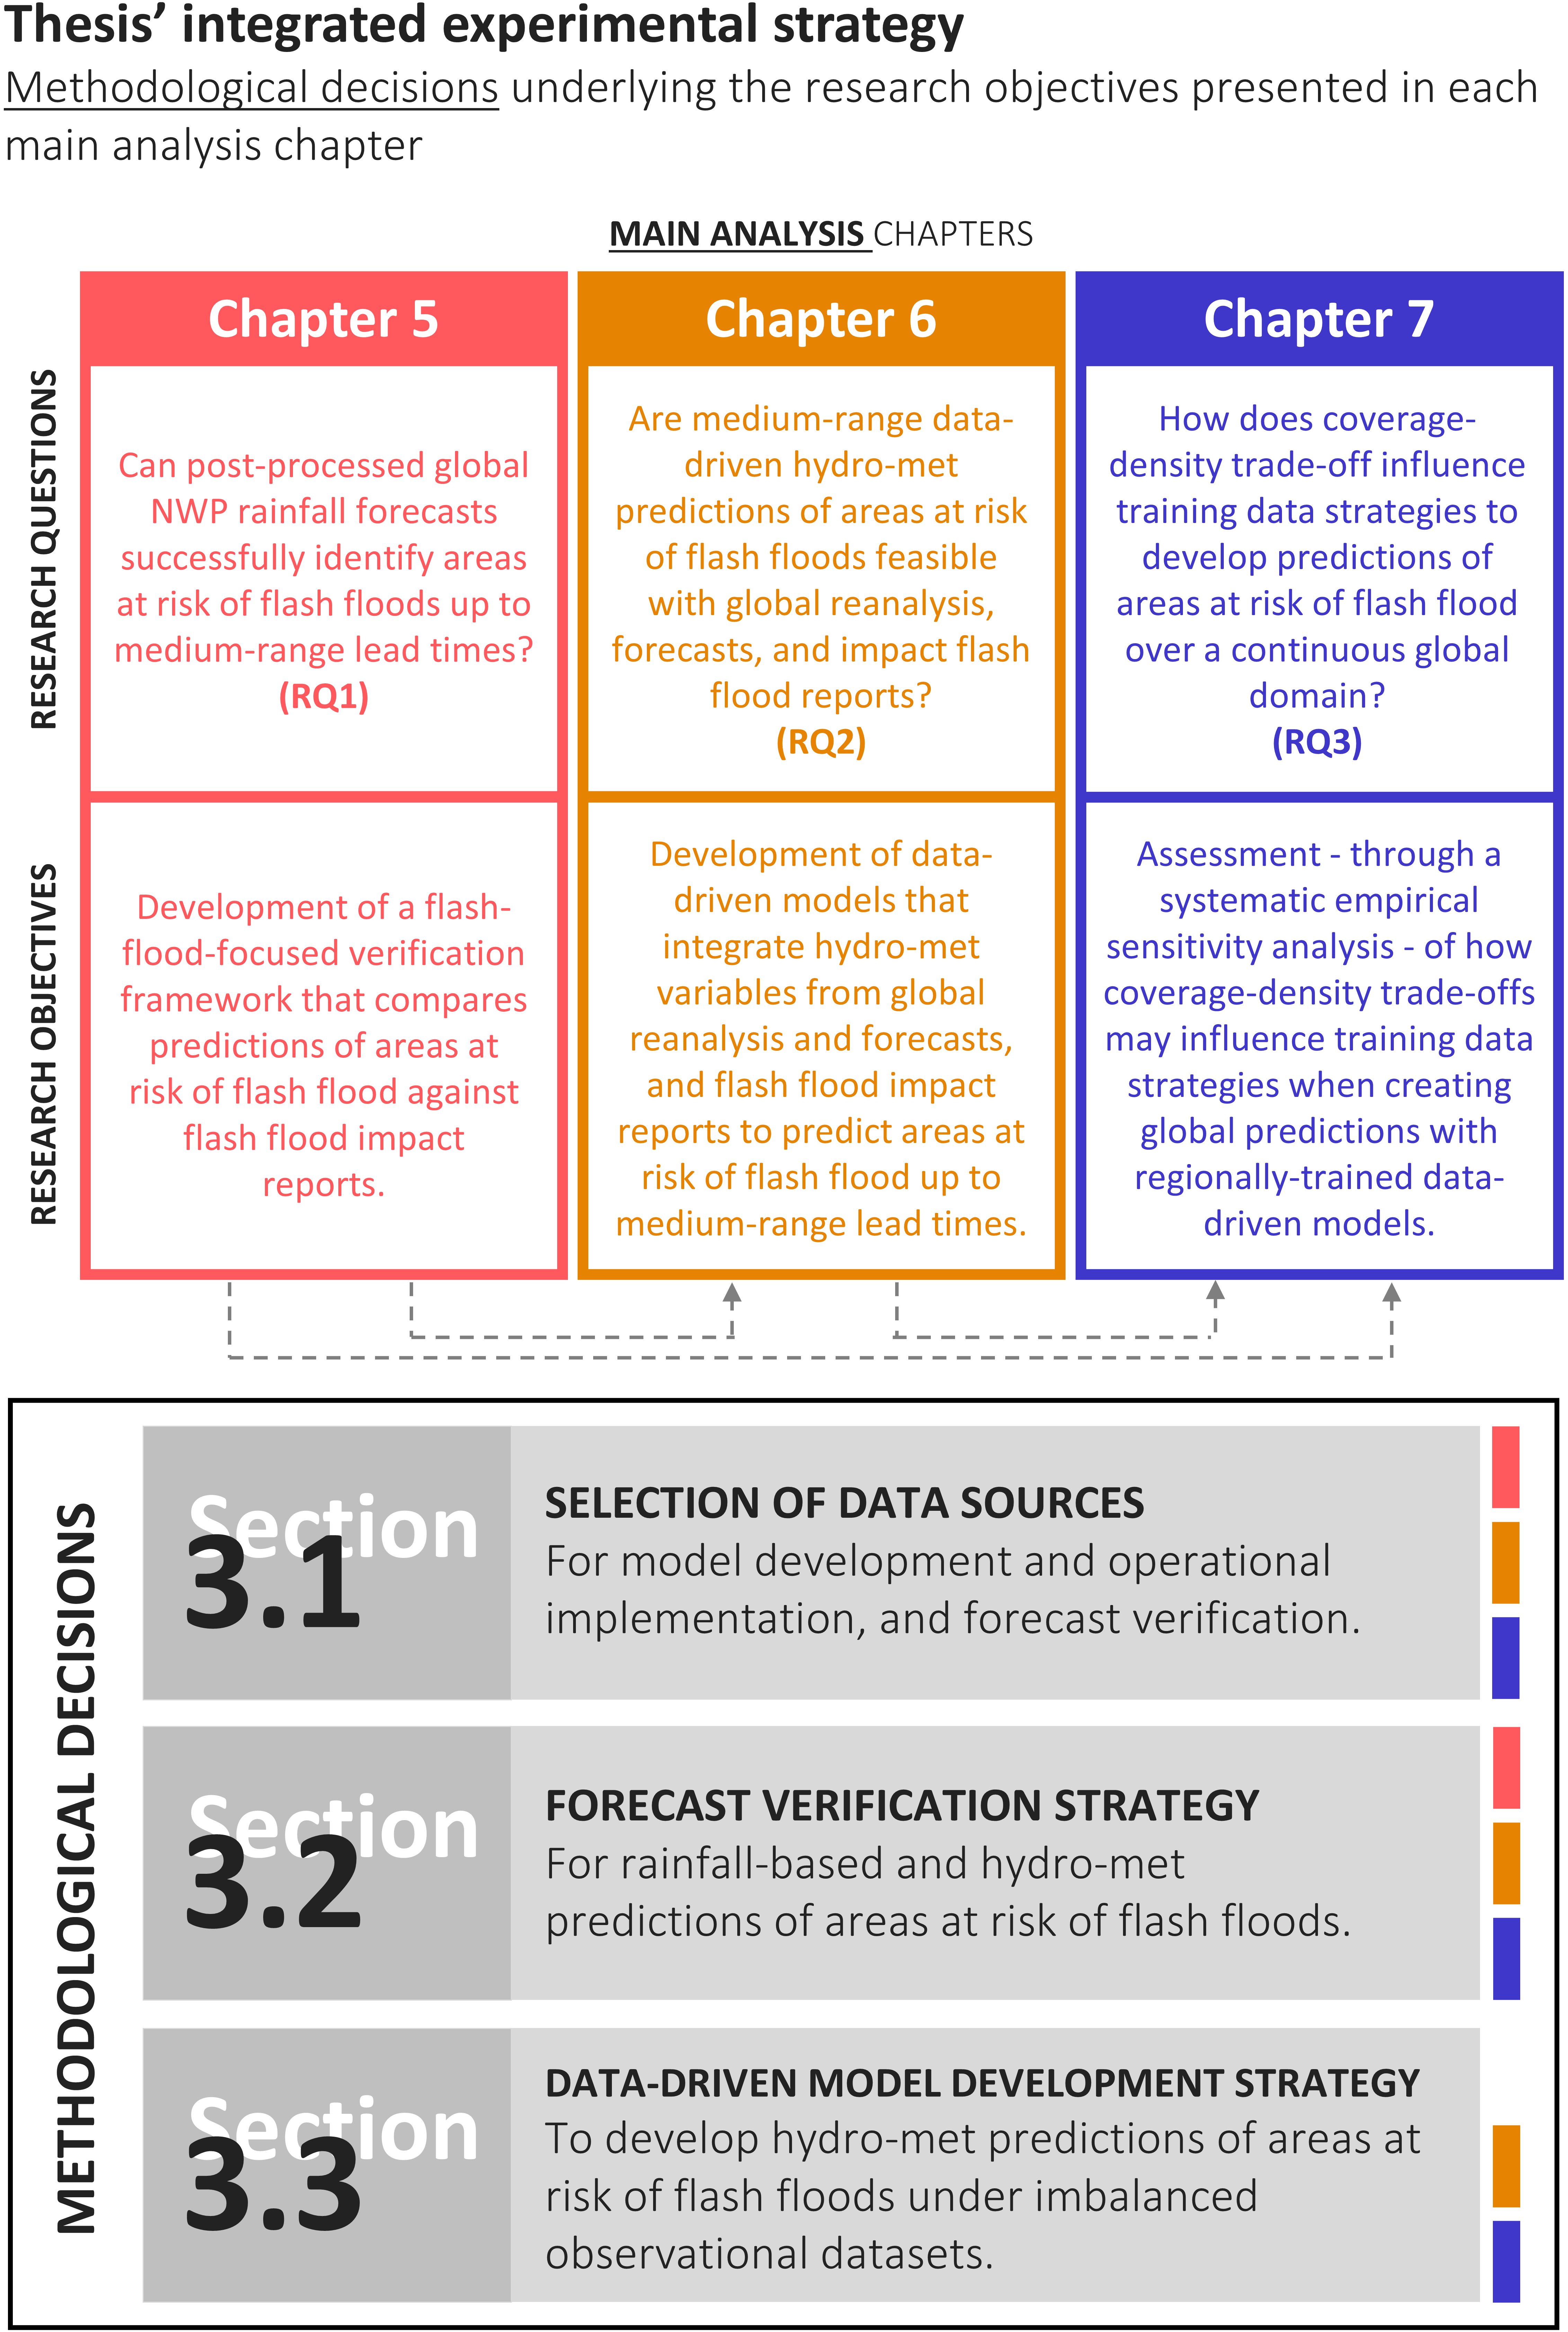
\includegraphics[width=\textwidth]{chapter_03/figures/integrated_experimental_strategy.png}
\caption{\textbf{Thesis' integrated experimental strategy.} The infographic presents the hierarchical relationship between research questions (RQ1-RQ3), their corresponding research components, and underlying methodological decisions. The first row reminds the reader about the three research questions addressed in Chapters \ref{flash_flood_focused_verification_framework}, \ref{feasibility_PoFF}, and \ref{predictability_PoFF} (pink, orange, and purple cards, respectively) as introduced in Chapter \ref{general_introduction}. The second row outlines the research components developed to address each RQ. The cards maintain the chapter-specific colour coding. The horizontal arrows beneath the cards indicate the cross-chapter applications as introduced in Chapter \ref{general_introduction}, with colouration denoting chapters where components were employed. The third row (grey horizontal panels within the dashed grey box) identifies the three core methodological decisions that inform the experimental design: data source selection (Section \ref{experimental_data_requirements}), forecast verification strategy (Section \ref{experimental_design_verification_strategy}), and data-driven model development strategy (Section \ref{experimental_design_model_dev_imbalanced_data}). The coloured indicators on the right denote their application across the respective research components.}
\label{fig:integrated_experimental_strategy}
\end{figure}

The \marginpara{Second research component (addressing RQ2): development of short-range (day 1, reanalysis-based) hydro-meteorological, data-driven predictions of areas at risk of flash floods - Regional proof of concept over CONUS and global transferability assessment} second research component proposes a methodology to develop short-range (day 1, reanalysis-based) hydro-meteorological, data-driven predictions of areas at risk of flash floods. Due to data limitations, the methodology was developed over the CONUS. This data-driven approach represents a departure from traditional physically based hydrological modelling, which often struggles with computational demands and parameter uncertainty. In this second research component, a sensitivity analysis is also performed to assess which data strategy would be most suitable for extending the regional training globally, allowing predictions to be computed over a continuous global domain.

The \marginpara{Third research component (addressing RQ3): development of medium-range (up to day 5) hydro-meteorological, data-driven predictions of areas at risk of flash floods - Regional and global prototype} third research component extends the application of the data-driven model to medium-range forecasts, enabling the assessment of flash flood predictability beyond the typical day 1 lead time. This component applies the data-driven model developed in the second research component to longer-range NWP forecasts. It also applies the verification framework developed in the first research component to evaluate how predictive skill decays with increasing lead times. This evaluation is crucial for understanding the temporal limitations of actionable flash flood predictions.

The following sections outline the methodological decisions (Figure \ref{fig:integrated_experimental_strategy}, row related to the \textit{methodological decisions}) underlying each research component. These decisions encompass three primary areas: the selection of appropriate data sources (Section \ref{experimental_data_requirements}), the formulation of the forecast verification strategy (Section \ref{experimental_design_model_dev_imbalanced_data}), and the strategy for developing a data-driven model to identify areas at risk of flash floods under imbalanced observational datasets (Section \ref{experimental_design_model_dev_imbalanced_data}). 


%%%%%%%%%%%%%%%%%%%%%%%%%%%%%%%%%%%%%%%%%
\section{Data requirements and selection}
\label{experimental_data_requirements}

The development of a flash flood prediction system necessitates careful consideration of data requirements across all methodological components, i.e. model development, forecast verification (at different lead times), and future operational implementation. This section outlines the criteria for selecting the required data to develop a proof of concept of a system that produces medium-range forecasts of areas at risk of flash floods over a continuous global domain. 

\subsection{Criteria for data selection}

The selection of appropriate datasets must satisfy multiple criteria stemming from the distinct requirements of each research question, whilst maintaining consistency across the integrated experimental design of this thesis.

\subsubsection{Observational data requirements}

Since \marginpara{Observational data requirements n.1: spatio-temporal accuracy of reported flash flood events} flash floods are very localised events, happening in small catchments, there is a need for flash flood observational datasets that report accurately the location and time of flash flood occurrence, and the spatio-temporal uncertainty around each recording. Such precision is essential for developing a robust flash-flood-focused verification framework (as in RQ1), where grid-based assessments demand an accurate spatial assignment of events to model grid cells. For RQ2 and RQ3, such accurate spatio-temporal information enables prediction systems (whether data-driven or physics-based) to capture the relationship between local meteorological conditions and flash flood occurrence, accounting for the fine-scale processes that govern these rapid-onset events.

The \marginpara{Observational data requirements n.2: long, complete, and consistent timeseries of reported events.} rarity of flash flood occurrence necessitates an extensive temporal coverage of observational timeseries to accumulate an adequate number of flash flood events across multiple years for robust forecast verification (as in RQ1, RQ2, and RQ3) and for machine learning model training purposes (as in RQ2). Moreover, systematic reporting standards across the spatial domain ensure unbiased verification and prevent the introduction of artificial patterns during model training.

\subsubsection{Hydro-meteorological forecasts requirements}

The \marginpara{Hydro-meteorological forecasts requirements n.1: consistency over different lead times} transition from short-range forecasts (day 0 to 1, as analysed in RQ1 and RQ2) to medium-range forecasts (up to day 5, as analysed in RQ1 and RQ3) requires the adoption of a system capable of providing forecasts across the entire lead time horizon. Such consistency is fundamental as the introduction of different forecasting systems (e.g. one - lower resolution - for training and one - higher resolution - for forecast production) would compound extrinsic uncertainties into a system characterised by substantial intrinsic uncertainties stemming from the chaotic nature of atmospheric processes and the complexity of flash flood generation mechanisms. Hence, by considering a system capable of providing forecasts over all required lead times, model performance degradation with lead time might reflect closely genuine predictability limits of flash flood prediction rather than dataset inconsistencies.

Due \marginpara{Hydro-meteorological forecasts requirements n.2: capability to represent flash-flood-triggering rainfall events} to their coarse resolution and parametrisation schemes of convective systems, raw global NWP model outputs systematically underestimate localised rainfall extremes, which are critical for flash flood generation. Consequently, both the verification of areas at risk of flash floods (as in RQ1, RQ2, and RQ3) and the training of machine learning models for the prediction of such areas at risk of flash floods (RQ2) require rainfall estimates capable of identifying flash-flood-triggering rainfall events. 

Whilst \marginpara{Hydro-meteorological forecasts requirements n.3: Global coverage} the proof of concept proposed in this thesis focuses in the creation (as in RQ2 and RQ3) and verification (as in RQ1, RQ2, and RQ3) of predictions of areas at risk of flash floods over the CONUS, the methodology must support global extension. This requirement necessitates globally consistent datasets without regional discontinuities, typically provided by global NWP model outputs.


\subsection{Available Data Sources and Final Selection}

\subsubsection{Observational data}

The choice of an impact-based database rather than hydrological measurements reflects the fundamental nature of flash floods as localised phenomena occurring predominantly in ungauged catchments. Traditional gauge-based observations fail to capture the majority of flash flood events due to their sparse spatial distribution and the rapid onset characteristics of these events \citep{Gaume_2009, Gaume_2016}. Although subject to reporting biases - for example, due to population density \citep{Marjerison_2016}, impact databases provide a more feasible approach for continental-scale (and subsequent global scale) forecasts development and verification, where the installation and maintenance of denser observational networks remains economically and logistically prohibitive.

This study utilises the Storm Events Database, maintained by NOAA, as the primary source of flash flood observations across the CONUS. This database represents the most comprehensive and systematically maintained record of flash flood impacts available at a continental scale, containing detailed spatio-temporal information for events from 1950 to the present (purple area in Figure \ref{fig:workflow_verif_framework}). Alternative options include the ESWD database, maintained by ESSL, that provides reports on severe weather across Europe. Two main issues arise with this database. First, it does not provide direct reports of flash flood events. It provides reports of "extreme rainfall", which are considered as a proxy for flash flood events. However, as stated in Chapter \ref{general_introduction}, there is no always a direct correlation between rainfall events and flash flood generation. Second, the clear spatial bias, with more reports from Germany (where ESSL is based), would introduce errors in the training and verification of predictions for areas at risk of flash floods.

The Storm Events Database offers several advantages that justify its selection\footnote{For more details on the Storm Event Database, the reader might want to refer to Section \ref{storm_event_database}}. First, it provides consistent reporting standards across all US states, enabling uniform analysis across diverse hydro-climatic regions. Second, each report includes precise geolocation data, essential for grid-based verification approaches. Third, the database undergoes quality control procedures by NOAA, reducing, though not eliminating, reporting inconsistencies that might be present in other databases such as ESWD (with clear reporting biases over Germany). These characteristics make it the most suitable dataset for establishing a robust verification framework, acknowledging that similar approaches could be applied to other regional databases such as the European Severe Weather Database or global repositories like EM-DAT and DesInventar, each with their specific limitations and biases \citep{Panwar_2020}.

\subsubsection{Hydro-meteorological forecasts}

The selection of ERA5 and its post-processed variant ERA5-ecPoint reflects a deliberate strategy to maintain consistency across the different analyses in this thesis. ERA5-related datasets (both reanalysis and medium-range forecasts) were selected as they provide a long-term (from the 1940s - 1950s for ERA5-ecPoint - to the present), high-quality reconstruction of hydro-meteorological fields over a continuous global domain \citep{Hersbach_2020}. Thus, such a dataset can provide a consistent, long-term timeseries for training data-driven predictions of areas at risk of flash floods and their subsequent verification.

While ERA5 provides a consistent dataset for training over space and time, its coarse resolution (31 km) makes the raw ERA5 rainfall estimates inappropriate for flash flood applications, as localised rainfall peaks tend to be underestimated in the case of large-scale rainfall (whether from stratiform rainfall or large convective systems) or absent in the case of isolated convection. For this reason, the rainfall estimates used for training and verification in this analysis come from the post-processed ERA5 rainfall estimates with the ecPoint methodology, which provides a probabilistic distribution of how the localised extreme rainfall estimates might be within the model gird-boxes\footnote{A more detailed description of the ecPoint post-processing technique and the quality of ERA5-ecPoint rainfall reanalysis and forecasts can be found in Section \ref{ecpoint_rainfall}}.

Regarding the longer-range forecasts used to create the medium-range predictions of areas at risk of flash floods, it is common practice to fine-tune the training done with lower-resolution datasets (such as ERA5, at 31 km) to the higher resolution of more commonly used forecasting systems (such as ECMWF's IFS, at 9 km). In the field of data-driven weather forecasts, this is done in the AIFS which is trained over ERA5 and fine-tuned over the operational analysis at 9 km to obtain forecasts with a spatial resolution of \sim25 km  \citep{Lang_2024}. This approach was not adopted in this thesis because uncertainties related to such fine-tuning would be introduced in the forecasting chain, and it would be difficult to dissociate them from uncertainties in the predictability of the hazard itself related primarily to the physical processes that generate flash floods and the data used to create the short- and medium-range forecasts. Hence, the long-range forecasts from ERA5 (i.e. model runs beyond day 0, which correspond to the better-known reanalysis dataset) and its corresponding ecPoint post-processed rainfall estimates were used in this thesis\footnote{The reader is referred to section \ref{datasets_era5} and \ref{ecpoint_rainfall} for a more detailed description of the ERA5 hydro-meteorological forecasts}. 

Traditional \marginpara{Evaluation metrics for model development} loss functions weigh all misclassifications equally, effectively obscuring the importance of correctly identifying rare positive events. In some contexts, the cost of missing an event might exceed that of a false alarm, while in others, the opposite might be more of a concern due to scarce resources for preparedness ahead of an event and emergency management during the event. Hence, during the development of data-driven predictive models (as in RQ2), approaches that reflect this asymmetry must be considered, such as identifying suitable evaluation metrics for model development. 

Moreover \marginpara{Evaluation metrics for forecast verification}, during verification, it might not be possible to understand whether forecasting systems overestimate the frequency of flash flood events due to intrinsic biases in the predictive model or due to the underrepresentation of the hazard occurrence. Performance metrics suitable for balanced datasets become misleading with extreme imbalance. Hence, the use of appropriate verification metrics, such as the combination of precision and recall, might be able to capture meaningful predictive signals of yes-events (cases indicating the occurrence of flash floods).


%%%%%%%%%%%%%%%%%%%%%%%%%%%%%%%%%%%%%%%%%
\section{Forecasts verification strategy}
\label{experimental_design_verification_strategy}
















%%%%%%%%%%%%%%%%%%%%%%%%%%%%%%%%%%%%%%%%%%%%%%%%%%%%%%%%%%%%%%%%%%%%%%%%%%%%%%%%%%%%%%%%
\section{Data-driven model development strategy under imbalanced observational datasets}
\label{experimental_design_model_dev_imbalanced_data}

The development of data-driven flash flood prediction models must confront the fundamental challenge of extreme class imbalance in observational datasets, stemming from the rarity of events and the underrepresentation of flash flood occurrences in observational timeseries \citep{Gaume_2009, Panwar_2020, Marjerison_2016}. Flash flood events represent approximately 0.2\% of the observational dataset, creating one of the most severe class imbalance problems encountered in environmental prediction, similar to, for example, lightning detection problems \citep{Cavaiola_2024}. This section outlines the strategies employed to address these challenges while ensuring robust and generalisable predictions.

Such \marginpara{Algorithmic convergence to trivial solutions} an imbalance towards non-events (cases indicating the non-occurrence of flash floods) poses significant challenges for machine learning algorithms, which may converge to trivial solutions that never predict positive events. These trivial classifiers achieve an accuracy greater than 99\% by simply predicting non-events for all cases, yet provide no operational value. The challenge lies in developing models that can identify the subtle signals preceding rare events without being overwhelmed by the preponderance of negative cases.

Ensemble \marginpara{Ensemble learning techniques} learning techniques also offer a valid approach to address the class imbalance problem. Unlike data-level approaches that modify the training dataset through over- or under-sampling, ensemble methods preserve the original data distribution whilst improving minority class detection through algorithmic diversity. This choice reflects a deliberate decision to maintain the integrity of the observational dataset, avoiding the introduction of synthetic samples or the loss of potentially informative negative examples. The experimental design incorporates multiple ensemble algorithms, including Random Forest, Gradient Boosting variants (XGBoost, LightGBM, CatBoost), neural networks, and ensemble stacking. Each algorithm offers different mechanisms for handling imbalanced datasets. For example, random forest creates multiple views of the data through bootstrap sampling, where positive events may be better represented in individual trees. Gradient boosting methods sequentially focus on misclassified examples, progressively improving detection of difficult-to-predict positive cases. This diversity enables a comprehensive assessment of which algorithmic approaches best suit the flash flood prediction challenge. Moreover, ensemble methods combine predictions from multiple base learners, each potentially capturing different aspects of the flash flood generation process. This diversity provides robustness against the instabilities that can arise when training individual models on severely imbalanced data.



%%%%%%%%%%%%%%%%%
\section{Summary}

This chapter has articulated an integrated experimental design that systematically addresses the challenge of producing medium-range predictions of areas at risk of flash floods across a continuous global domain. The methodological framework illustrates how seemingly distinct research components converge into a coherent strategy, with each element carefully chosen to support the overarching research questions in this thesis. This integrated design acknowledges that flash flood prediction represents a cascade of uncertainties. By maintaining methodological consistency whilst allowing component-specific optimisation, the framework provides a robust platform for advancing operational flash flood prediction capabilities. The subsequent \textit{Main Analysis} chapters (\ref{flash_flood_focused_verification_framework} to \ref{predictability_PoFF}) will implement this experimental design, progressively building from fundamental verification principles through regional model development of short- and medium-range forecasts, to the extension of predictions over a continuous global domain.